\section{Algorithm outline}
\label{section:algorithm}

contact 
forces
dynamics/rotation/timestep
 
\begin{algorithm}
 
   Blueprint of explicit DEM code's overall structure.
 
 \label{algorithm:dem-blueprint}
% \SetAlgoNoLine
 \begin{algorithmic}[1]
   \For{$t < T$}
   
	\For{i = 0 to N triangles}

		\For {j = i+1 to N triangles}
				
			\State $distance = TTD(i,j)$
				
			\If{(distance $<$ margin) AND ParticleID(i) != ParticleID(j)}

				\State $contact(PID(i)).add(point, normal)$

			\EndIf
			
		\EndFor
			
	\EndFor


	\For{z = 0 to NB particles}

		\For {k = 0 to contacts(z).size()}

			\State $force = granular(velocity(z), position(z), contacts(z).getcontact(k))$

		\EndFor
	
	\EndFor    
    
     \State $t \gets t + \Delta t$
   \EndFor   

 \end{algorithmic}
\end{algorithm} 


We focus on DEM with explicit time stepping (Algorithm \ref{algorithm:dem-blueprint}). 
A straightforward implementation consists of one outer time stepping loop
hosting three inner loops. 
The first inner loop detects contact points between particles' triangles and
check each triangle vs.~the others.
It thus has to loop over the particles.
The second loop runs over these contact points and translates them into forces.
While contact points could in principle be translated into forces straightaway,
it makes sense to outsource the force computation into a separate algorithm
phase.
The third loop applies the forces to the particles and updates the particle
positions.
It has to loop over all particles.


{\bf Contact detection.}
We employ a visco-elastic particle model with spring forces here, where the
actual particle is incompressible.
However, it is equipped with a small halo layer of size $\epsilon >0$:
While the particles are rigid bodies, two particles are assumed to contact each
other if their distance is smaller than $2\epsilon$. 
However, the distance always is positive.
Such an approach equals a Minkowsi sum approach where the actual particles are
blown up by a circle with radius $\epsilon$ and may penetrate each other up to
depth of $\epsilon $.


\begin{figure}[htb]
  \begin{center}
    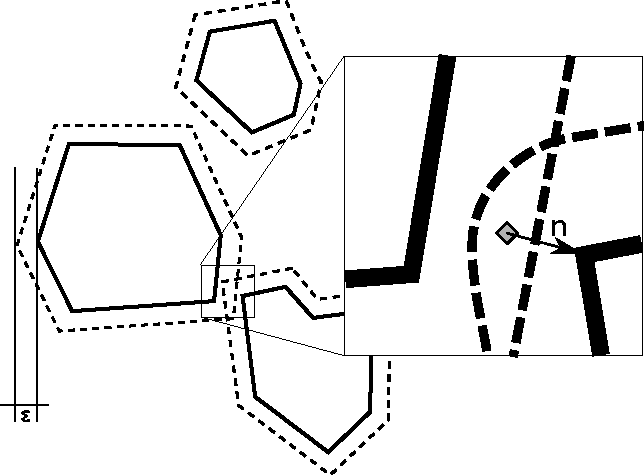
\includegraphics[width=0.45\textwidth]{sketches/minkowski.pdf}
  \end{center}
  \caption{
    Left: Three particles with their $\epsilon $ environment. The particles do
    not penetrate each other, but two particles plus their $\epsilon $
    environment penetrate and create one contact point with a normal. 
  }
  \label{figure:minkowski}
\end{figure}

As we apply a solid particle model, contact always is a unique point. 
We define it to be the centre of an overlap region (Figure \ref{figure:minkowski}), i.e.~the
distance $d$ between a particle $A$ and its contact point with a second particle
is $0 < d \leq \epsilon$.
Each contact point is equipped with a normal $n$ pointing from the contact point
to the surface of the contacting body's surface.
As the distance is positive, the normal is well-defined and we have $|n| \leq
\epsilon $.
Please note that the normal direction depends on whether we make particle $A$
being hit by particle $B$ or the other way round: each normal associated with a
particle points along the outer normal of the body.
Despite the fact that we employ a rigid body model, multiple contact points
between two bodies may exist as particles may be concave and their Minkowsi sum
may overlap.


For two given particles $A$ and $B$ with corresponding sets of triangles
$\mathbb{T}_A$ and $\mathbb{T}_B$, the contact detection thus reads:
Loop over all triangle pairs $t_i \in \mathbb{T}_A, t_j \in \mathbb{T}_B$ and
identify those pairs that are closer than $2\epsilon $.
For those close, determine the middle point along the closest distance. 
The point equals the contact points while the distance vector identifies
its normal.
Add the contact point to a contact point set $\mathbb{C}_A$ and to the set
$\mathbb{C}_B$.
The normal in the latter is inverted.
Such an algorithm has the complexity $\mathcal{O}( | \mathbb{T}_A| \cdot
|\mathbb{T}_B|)$ and makes the overall naive implementation a member of 
$\mathcal{O}( | \mathbb{T} |_{max}^2  )$ if $| \mathbb{T} |_{max} )$
is the maximum number of triangles per particle.


{\bf Force model.}
We apply the linear spring-dashpot force model from Cundall and
Strack \cite{19,Samiei} to study the efficiency of our implementation.
Per particle $A$, it accumulates all contact points in $\mathbb{C}_A$ into one
translational and one rotational repulsive force with some damping.
We make $\mathbb{C}_A$ subject to a postprocessing which eliminates all
collision point duplicates which is all duplicates that are closer than
$min(h_{A,min},h_{B,min})$. 
It is the smallest face length of the meshes representing $A$ and $B$.
No contact point may be closer than this value.
On the preprocessed contact point set $\mathbb{C}_A$ we then determine
\begin{eqnarray}
%   f_{trans} = \sum _{c \in \mathbb{C}_A} 
%   -k_{repulsive} (\epsilon - |n|) \frac{n}{|n|}
%   \\
  f_{trans} = \sum _{c \in \mathbb{C}_A} 
  \min \left( 0, -k_{repulsive} (\epsilon - |n|) + k_{damp}
  \frac{(v_B-v_A,n)}{|n|}  \right) \frac{n}{|n|}
  \label{equation:forces:translational}
  \\
  f_{rot} = \sum _{c \in \mathbb{C}_A}
  \label{equation:forces:rotational}
\end{eqnarray}

%What are the expensive phases 
\noindent
$k_{repulsive}$ and $k_{damp}$ are material coefficients. 
We use the normal's norm to determine the model's penetration depth, while the
change rate of this depth is derives from the projection of the relative
velocity between the two particles onto the normal vector.
We use the the particles' velocities $v_A$ and $v_B$ here.
The $\min $ function ensures that the force always pulls particle away from each
other. 
There is no particle attraction.


Our Newtonian DEM code relies solely on pair-wise interactions so far. 
With a modifcation of
($\ref{equation:forces:rotational}$,$\ref{equation:forces:rotational}$), it is
however possible to introduce more sophisticated force patterns.
We note that the complexity of the force computation depends solely on the size
of $\mathbb{C}$ if we anticipate that we have to run over all particles to
update their position in space due to momentum anyway.
$\mathbb{C}$ typically is very small if particles are of reasonably the same
size. 
If particle sizes vary dramatically, comparably large particles experience
contact forces from many small particles.
In this case, there are however few large particles compared to the overall
number of particles.


{\bf Time stepping.}
For the present work, we rely on an explicit Euler as simplest time stepping
scheme possible.
We implement a symplectic scheme where the velocity is updated with the forces
before the position is updated with the new velocity \cite{Samiei,37}. 
While the extension to implicit schemes is beyond scope \cite{xxx}, our outlook
does discuss more sophisticated and adaptive time step choices which translate
the present time-driven scheme into an event-driven algorithm \cite{xxx}.

